\section{Quick tutorial}

In this section we are going to guide you through a simple tutorial. After you finish all the steps described here, you will have
a basic understanding of what you can do with the \emph{Reprotool IDE}. However, we will not delve deeply into the logic behind these
steps here, this is just a basic tutorial for you to get a general idea about \emph{Reprotool}. You will find more detailed information
about the steps performed in this tutorial in later chapters that are devoted to a single topic.

\subsection{Prerequisites}

We assume you have already successfully completed the steps in the previous chapter that shows you how you can import external textual
use-case specifications into the \emph{Reprotool} project. More precisely, we assume you have the \emph{Admission system} exmaple
project installed in your workspace and the \emph{admission.swproj} project already contains the use-cases specified in the \emph{data}
directory.

\subsection{Outline of the tutorial}
\begin{enumerate}
  \item We will add annotations to some use-case steps in the project.
  \item We will run the model check of annotation semantics in our project.
  \item We will show a counter-example trace of the model checker output.
  \item We will fix the annotation inconsistency in the project.
\end{enumerate}

\subsection{Add annotations to the project}

Open the \emph{admission.swproj Reprotool} project by double-clicking it in the project explorer of the \emph{Reprotool IDE}. This project
file is located in the \emph{Admissions system} project that is already installed in your workspace. Now, double-click the
\emph{Register in the system} use-case. A new use-case editor instance will open. In the use-case editor, click on the use-case step with
label \emph{1}. Now press CTRL + 4 on your keyboard. This will add a new annotation to the
selected step. You will notice a small black triangle in the label field of the selected use-case step. If you click on it, the
annotation will be shown. Click on the annotation and display the \emph{Properties view}. There are 2 fields that you need to fill there.
Type \emph{resource} as \emph{Id property} and select \emph{Temporal annotation create} as the \emph{Annotation type property}. 
You can view this situation in the next figure:

\begin{figure}[ht]
  \centering
  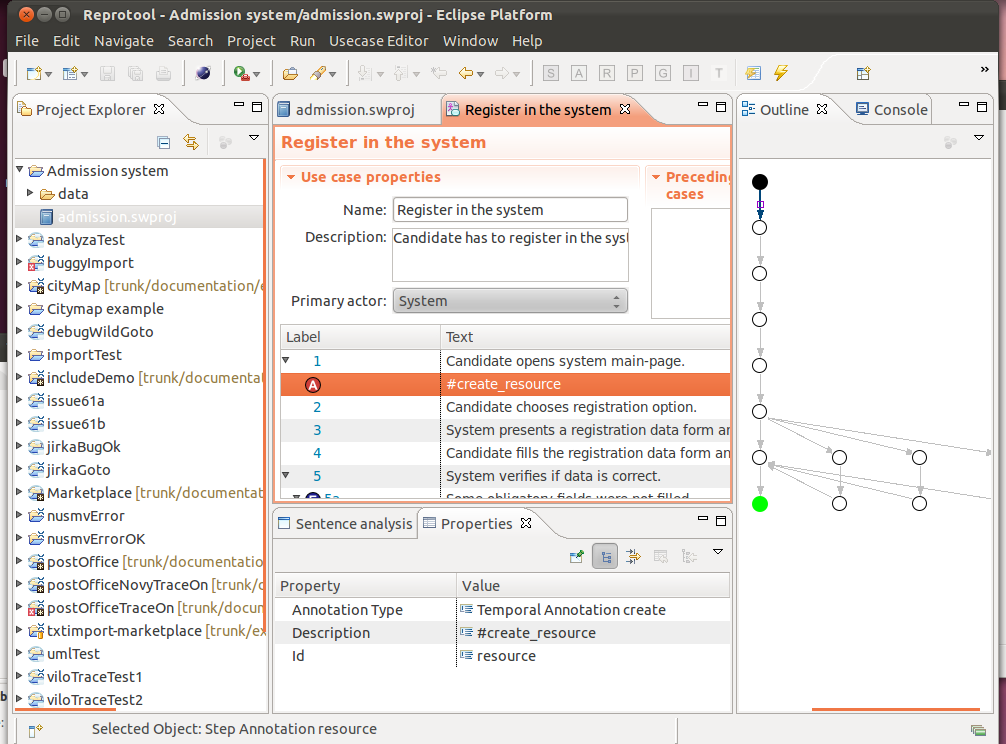
\includegraphics[height=280pt]{images/reprotoolQuickTutorial1}
  \caption{Adding annotations screen}
  \label{fig:reprotoolQuickTutorial1}
\end{figure}

Now use the same steps to add the \emph{use} annotation with id \emph{resource} to some step in the use-case \emph{Print application}.
In this tutorial we use two predefined annotations \emph{create} and \emph{use}. These annotations have predefined meaning in default
\emph{Reprotool} projects. You are however free to change this meaning and to add new annotations. One of the rules that binds the
usage of the \emph{create} and \emph{use} annotations is this:

\begin{enumerate}
 \item After \emph{create} there must be some branch containing \emph{use}.
\end{enumerate}

As you will see later, this rule does not always hold true in our project so the model checker will generate a counter-example that
shows us the case where the rule is violated. After you have set the second annotation, you should end up with a screen similar to this:

\newpage

\begin{figure}[ht]
  \centering
  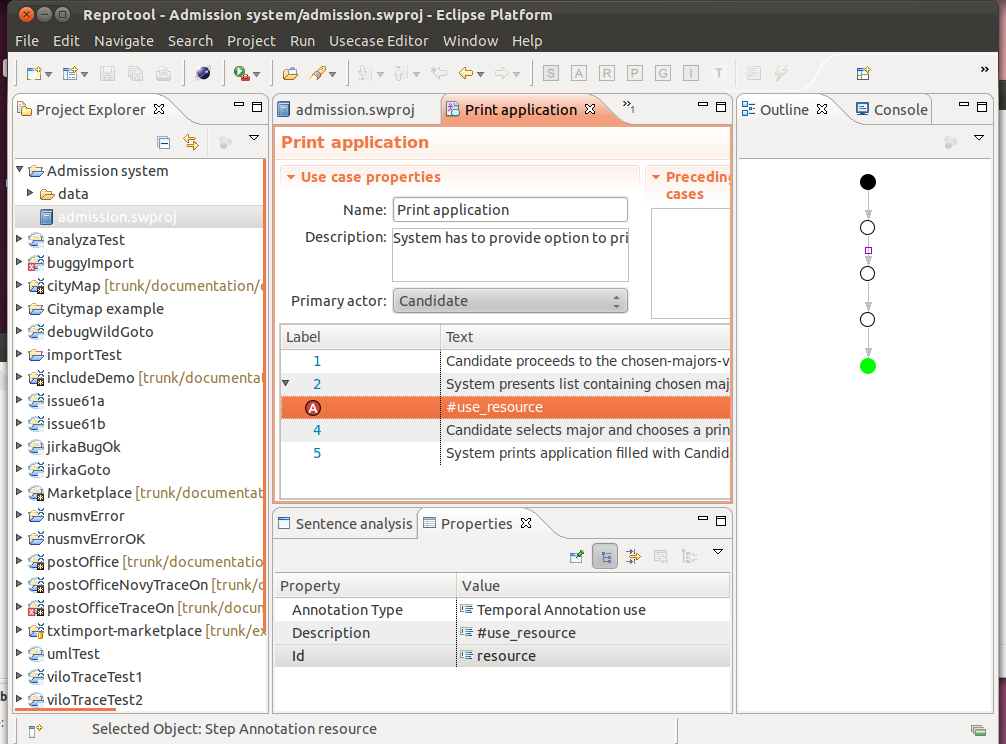
\includegraphics[height=280pt]{images/reprotoolQuickTutorial2}
  \caption{Adding annotations screen}
  \label{fig:reprotoolQuickTutorial2}
\end{figure}

\subsection{Run the model checker}
Right-click the \emph{admission.swproj} file in the project explorer and run the \emph{Convert SW project to SMV} command from the
context menu. A new file with name \emph{admission.swproj.nusmv} will be generated in the project. Double-click it in the project
explorer to display it. You might be asked if you want to add the \emph{Xtext nature} to the project \emph{Admission system}. Choose yes.
What you see there is the model checking specification of our project for the \emph{NuSMV} model checker. To run the \emph{NuSMV} model
checker, right-click the file \emph{admission.swproj.nusmv} and run the command \emph{Run NuSMV Verification}. The model-checker trace
will be printed on the console and you can notice in the project explorer that a new file named \emph{admission.swproj.cexmp} has been
generated.

\subsection{Display the counter-example trace of the NuSMV model checker}

Double-click the \emph{admission.swproj.cexmp} file in the project explorer and make sure the outline-view is displayed. We will not go
here into the details how to read the counter-example trace. For now, just notice you can select in the outline view a red arrow and the
corresponding step will be selected in the editor view. It also works in the opposite direction. Also notice the properties view, which
contains quite a lot of important information when reading the counter-example. This situation is depicted in the next figure:
\begin{figure}[ht]
  \centering
  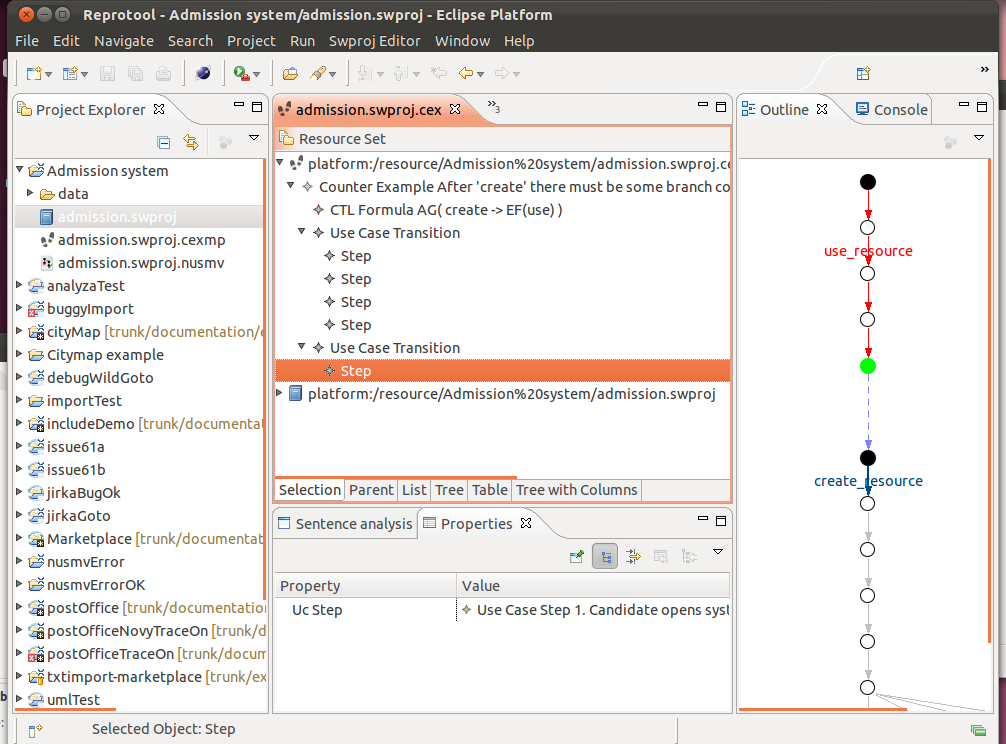
\includegraphics[height=280pt]{images/reprotoolQuickTutorial3}
  \caption{Model checker counter-example trace}
  \label{fig:reprotoolQuickTutorial3}
\end{figure}

\subsubsection{The idea how the model checker performes verification}
The model checker sees a number of use-cases in our project. And it tries to run all of them in any possible order. But every use-case
is run only once. In every step of the simulation, it observes if any of the temporal logic properties imposed on the project has been
violated. By adding annotations to the steps in \emph{Reprotool} project, you impose new restrictions that are checked by the model
checker.

\subsubsection{Explanation of the violated property}

Firstly, let us remind the rule that has been violated:

\begin{enumerate}
 \item After \emph{create} there must be some branch containing \emph{use}.
\end{enumerate}

And now, let us remind what annotations we have added to the \emph{Admission system} project. We have added the \emph{create\_resource}
annotaion to the \emph{Register in the system} use-case and we have added the \emph{use\_resource} annotaion to the
\emph{Print application} use-case. In case the use-case \emph{Register in the system} is executed \emph{before} the
\emph{Print application} use-case, then the property is not violated. (Remember all of the use-cases are run exactly once, so if
the use-case \emph{Register in the system} is currently being executed and the use-case \emph{Print application} has not yet been
executed, we know it \emph{will} be sometimes executed and the property holds true.)

However, on the other hand: If the use-case \emph{Print application} is executed before the \emph{Register in the system} use-case, then things
are different: When the use-case \emph{Register in the system} is being executed and the use-case \emph{Print application} has been
already executed, we know for sure that this use-case will not be executed in the future. And that is why we know the \emph{use\_resource}
annotation will not appear in the future, thus the property is violated.

\subsection{Fix the annotaion inconsistency}

One of the possible ways how to fix the inconsistency, is to specify that the \emph{Register in the system} use-case \emph{preceds} the
\emph{Print application} use-case. It is possible to specify the precedence relations already in the textual use-case specifications,
but now we are going to do it manually. In the counter-example trace, double click in the outline-view some step of the first use-case.
The use-case editor with the selected use-case \emph{Print application} will fire up. Now click the icon in the
\emph{Preceding use-cases} area and add the \emph{Register in the system} use-case to the list of the use-cases that precede the
\emph{Print application} use-case. Save the project and run the model checking again. Notice in the console output that all specifications
are true. Also notice no counter-example has been generated this time.